\chapter{samaseyxya suLiyalilx}

bAla subarxhamxNayxmfge gaNita eMdare hecucx Asakitx yArAdarU shikaSxkaru rajada meVle idadxre muKayx shikaSxkaru ivaranunx A taragatige kaLuhisutitxdadxru. mAsatxru A taragatige hoVdare reVKAgaNitakekx saMbaMdhisidaMte kelavu parxshenxgaLanunx keVLuvudu. anaMtara kapupx halageya meVle kelavu citarxgaLanunx baredu parxmeVyagaLa AdhArada meVle Akaqtiyalilx kelavu koVnagaLa parimANavanunx keVLutitxdadxru. vidAyxthiRgaLu parxmeVyagaLanunx jAcnxpisikoMDu utatxrisutitxdadxru.
\begin{figure}[H]
\centering
\includegraphics[scale=0.7]{src/figures/m_179a.eps} 
\end{figure}
citarxdalilx $A\hat{C}B$ da parimANaveVnu? eMdu keVLida takaSxNa umeVsha $90^\circ$ eMdu heVLida heVge? eMdaru athaRvaqtatxda paridhikoVna $90^\circ$ alAvx sArf eMda. mAsatxru matotxMdu citarx baredaru.
\begin{figure}[H]
\centering
\includegraphics[scale=0.7]{src/figures/m_179b.eps}
\end{figure}
citarxdalilx $A\hat{D}C$ da parimANaveVnu? eMdaru cakirxVya catuBuRjada horakoVna aMta sathxaBimuKa koVnakekx sama AdadxriMda $120^\circ$ eMdaLu naLini.
mAsatxrige saMtoVSavAyitu matotxMdu citarx baredaru
\begin{figure}[H]
\centering
\includegraphics{src/figures/m_179c.eps}
\end{figure}
citarxdalilx $y\times z$ koVnada parimANaveSuTx? eMdaru utatxra takaSxNa oMdeV baMtu $75^\circ$ eMdu. heVge eMdaru tirxBujada oMdu bAhuvanunx vaqdidhxsidAga uMTAguva horakoVna aMtasAthxBimuKa koVnagaLa motatxkekx sama. 
\begin{align*}
Y\hat{X}Z &=140^\circ-65^\circ\\
&=75^\circ
\end{align*}

mAsatxru matotxMdu citarx eLedaru.

\begin{figure}[H]
\centering
\includegraphics{src/figures/m_179d.eps}
\end{figure}
citarxdalilx $X$ matutx $Y$, $AB$ matutx $AC$ bAhugaLa madhayxbiMdugaLu $BC=8$ seMmiV Adare $xy=?$ eMdaru gwri kapupxhalageya hatitxra baMdu. tirxBujada eraDu bAhugaLa madhayx biMdugaLanunx seVrisuva saraLa reVKeyu mUraneya bAhuvige samAnAMtaravAgirutatxde. matutx adara adhaRdaSiTxrutatxde AdadxMriMda $xy=4$ seM.miV eMdaLu bAla subarxhamxNayxmfge nAnu keVLida elalx parxshenxgaLigU vidAyxthiRgaLu utatxra heVLeV biTaTxralalx. anonxV saMtoVSadalilx matotxMdu citarx baredu oMdu gotAtxda koVnada parimANa eSuTx eMdu keVLidaru.
\begin{figure}[H]
\centering
\includegraphics{src/figures/m_181.eps}
\end{figure}

\begin{center} 
citarxdalilx $AB=AC$
$$
\begin{matrix}
O\hat{B}C &=60^\circ & \quad  O\hat{C}B &=50^\circ\\
D\hat{B}O &=20^\circ & \quad O\hat{C}E &=30^\circ\\
O\hat{D}B &=50 & \quad O\hat{E}C & =40^\circ\\
\end{matrix}
$$
$D\hat{A}E =20^\circ$
\end{center}

hAgAdare $DAE$ koVnada parimANaveVnu? eMdaru taragati nishashxbadhxvAyitu. vidAyxthiRgaLu eSuTx parxyatinxsidarU avarige tiLiyalilalx. Aga mAsatxru idanunx mADi toVrisidaru.

$ABC$ \quad oMdu samadivx bAhu tirxBuja

$B\hat{A}C=20^\circ$ \qquad $\hat{B}=\hat{C}$
\begin{align*}
O\hat{B}C &=60^\circ  \qquad O\hat{C}B =50^\circ\\
\therefore O\hat{B}D  &=20^\circ  \qquad O\hat{C}E =30^\circ\\
B\hat{O}C &=70^\circ   \qquad D\hat{O}E =70^\circ\\
B\hat{D}O &=50^\circ   \qquad B\hat{O}D =110^\circ
\end{align*}

\begin{tabbing}
$D\hat{E}O=x$  \; \; Agirali \;\; $D\hat{O}E=70^\circ$ \;\; \= $\therefore$ \;\; $O\hat{D}E$ \= = \= $180^\circ-(70+x)$\\
\> \> = \> $180^\circ-70-x$\\
\> \> = \> $110^\circ-x$
\end{tabbing}
\begin{align*}
A\hat{E}D &=180-(40+x^\circ)\\
&=140^\circ-x\\
A\hat{D}E & =180^\circ-(140-x^\circ+20^\circ)\\
&=180^\circ-140+x^\circ-20^\circ\\
& =20^\circ+x
\end{align*}

Iga \quad $\bigtriangleup DEO$ \quad nalilx \quad $E\hat{D}O=110-x$, \quad $D\hat{O}E=70^\circ$ \quad $D\hat{E}O=x^\circ$

$x$ ge yAva belekoTaTxrU \quad $\bigtriangleup DEO$ \quad na koVnagaLu tiLiyutatxde. Adare \quad $\hat{x}$, \quad $o^\circ$ giMta jAsitx irabeVku.
